\subsection{ReG-Tries Implementation}
The ReG-Tries algorithm was first written in R. This choice was made for a few reasons. 
\begin{itemize}
\item{R has a wide range of graph theory, and brain networks related packages readily available. Many of these are packaged with the \emph{igraph} package.}
\item{R provides easy visualization of data. }
\item{Dependency issues. Many of the implementations of graph isomorphism algorithms have not been updated since the papers describing the algorithms were written. Thus many of them are dependent upon older software, and as a result, suffered dependency issues. On the other hand, the igraph package in R has graph isomorphism testing algorithms and canonical labeling (using \emph{bliss}) out of the box.}
\item{R functions as a scripting language, allowing easy data manipulations and prototyping}
\end{itemize}
In other words, R was chosen in order to provide a quick proof of concept, and easy integration for the purposes of this paper. 
There are several costs to choosing R to program the ReG-Tries algorithm. Unfortunately, this was not able to come to fruition.
%Negatives to choosing to program this in R.



\subsection{Data}
In recent years, projects have been developed to release large  brain connectivity datasets, called \textit{connectomes} to the public. Two notable projects are the 1000 functional connectomes project, and its successor the human connectome project. In the current study five hundred twenty functional connectivity matrices and 27 structural connectivity matrices were taken from the UCLA Multimodal Connectivity Database \cite{jesse11} which is part of the Human Connectome Project. The 520 functional connectivity matrices were taken from the ADHD200\_CC200 data set, which contains resting state fMRI connectivity data from 190 individials with ADHD (74 inattentive, 7 hyperactive/impulsive, and 109 combined subtypes) and 303 typically developing children between the ages of 7 and 21. Additionally, the scans were divided 208 by 3012 in the ratio of girls to boys. The 27 structural connectivity matrices were taken from the NKI\_Rockland data set. This set consisted of DTI tractography data from ``normal subjects,''. The structural connectivity datasets were later dropped from the analysis because of time constraints. 

\subsubsection{Processing}
The original matrices were weighted and undirected. Each connection matrix in the ADHD200\_CC200 data set had 190 vertices defined where each vertex corresponded to a predefined brain region. The ADHD200\_CC200 was obtained through the seeding method, so each edge is an estimate of the connection strength between predefined brain regions. The NKI\_Rockland connection matrices each had 188 vertices defined, where each represented a predefined tract region. Edges represented estimates of the densities of tract regions. 
In order for the connectivity matrices to be used for network motif discovery three steps were taken. Each connectivity matrix was processed using R (version 3.0.0). First, the data was normalized so that all values were between 0 and 1, where 0 would represent no connection, and 1 was the ``heaviest edge'' in the matrix.  Second, weak connections were removed according to thresholds. For functional connectivity data, an absolute threshold,  \ $t_{\alpha}$ between the values of 0 and 1 was applied, such that every value in our matrix below $t_{\alpha}$ would be removed. Third, the remaining values were binarized - that is - connections which were removed were converted to zeroes and remaining connections were converted to ones. These matrices could now be called undirected unweighted adjacency matrices: blueprints for undirected graphs. As such they were now suitable for analysis of network motifs.\\
\subsubsection{A unique approach to analyzing undirected motifs}
In the literature, as described by \cite{rubinov10} and exemplified by studies like \cite{deuker09} and \cite{wang09} only one prespecified threshold is applied to connectivity matrices to get unweighted data. This poses a problem, as graph theoretical measures are thus dependent on that one threshold. This is especially apparent as many of these studies cite previous studies on their decision of threshold - which makes both studies dependent on that threshold. The methodology of applying a range of thresholds has been suggested in the footnotes of \cite{sporns10}, but not used in research to this authors knowledge. Analysis can then be done on what properties are present in each of the thresholds - telling use what measures are present in the most highly connected portions of our network, and what properties are present only in specific networks. It is clear that properties held across multiple thresholds prove to be more present properties, and thus a stronger argument for their existence is gotten.\\
The use of multiple thresholds should provide a unique character to the network motif as well. Analysis of which motifs break down across the thresholds and which are still present gives us a more informative idea of the strength of a motif than at least one current method for producing weighted network motifs. In \cite{onella05}, Onella describes a technique for recording the \textit{intensity} of a network motif in a weighted network. Intensity is a measure of the average of all edge weights in a subgraph. What the problem with this is is that if a certain subgraph consistently has 1 edge which is heavily weighted, this will skew the whole motif to be labeled as more intense. With the methodology proposed here - if we look across increasing thresholds - we can give an estimate of where the connections are lost. We look at which motifs have decreased in frequency between thresholds, and which have increased in frequency. If we see, for example, a high frequency of pentagon subgraphs in one threshold, but see more path subgraphs on 4 vertices, we may be able to make an assumption - with other variables held constant that connections were lost from the pentagons between thresholds. This would provide a better character for the strength of a subgraph.\\
In the current study, 6 thresholds where 15, 30, 45, 60, 75, and 90\% of the weakest connections were removed were applied to each connectivity matrix (seen in figure 3).  
Because the ReG-Tries algorithm was never completed, analysis of motifs was done using the GTrieScanner software developed by Pedro Ribeiros (http://www.dcc.fc.up.pt/gtries/) on all connected subgraphs of order 3 and order 4 (see figure 1).
\begin{figure}
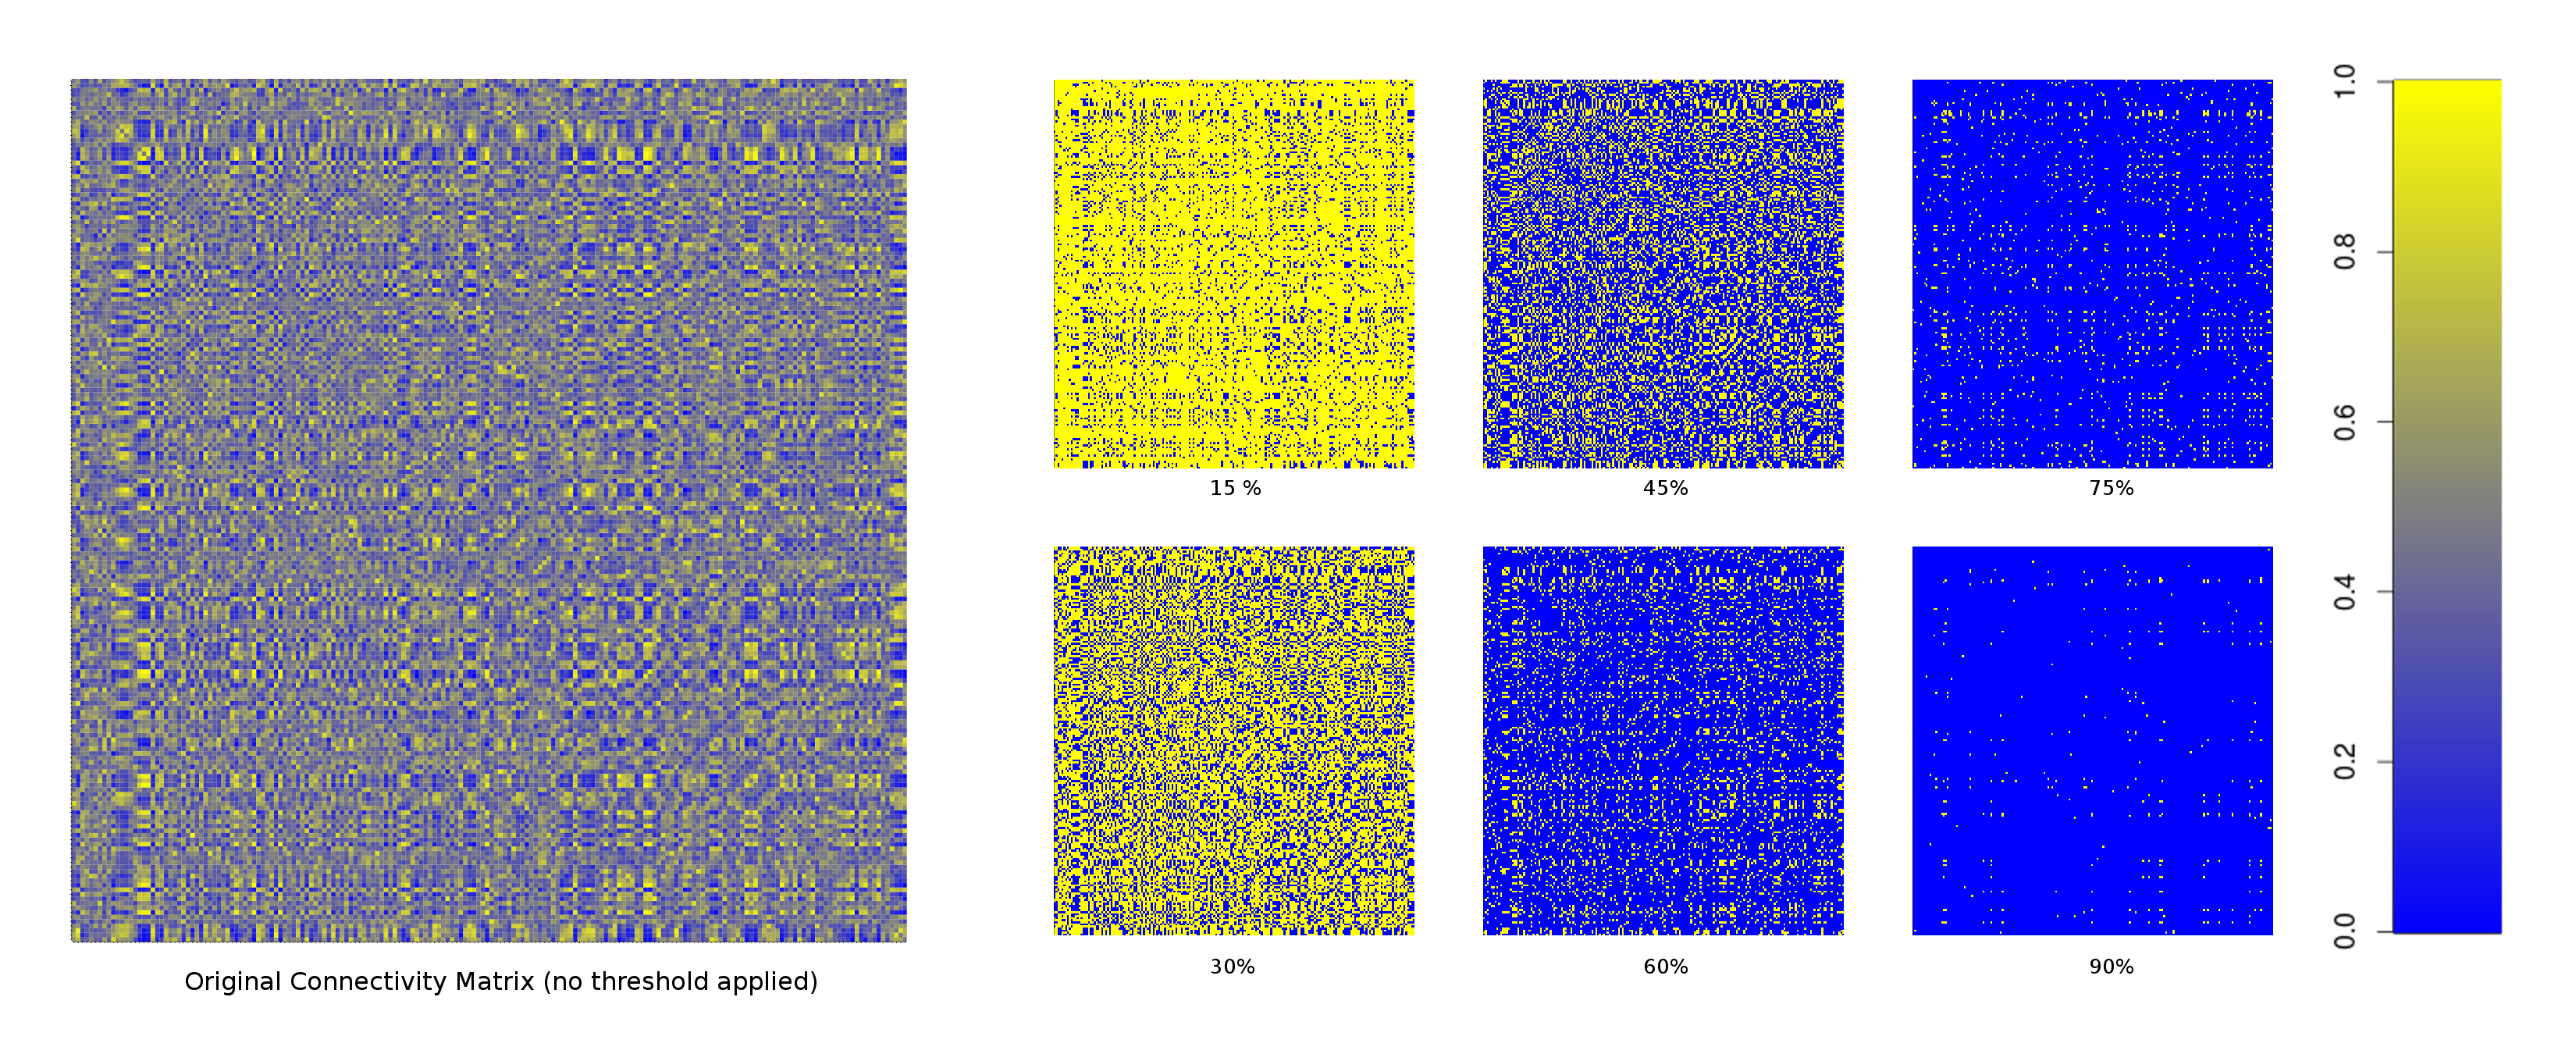
\includegraphics[width=\textwidth,height=\textheight,keepaspectratio]{figs/matrices.png}
\caption{A weighted connectivity matrix (left) with 6 thresholds applied to it (right).}
\end{figure}

\subsection{Comparison of Graph Isomorphism Algorithms}
Analysis of the performance of different graph isomorphism algorithms was originally planned as part of this study, but was never completed. A plan for a future study which follows through is described in the discussion. 